%%%%%%%%%%%%%%%%%%%%%%%%%%%%%%%%%%%%%%%%%
% Beamer Presentation
% LaTeX Template
% Version 1.0 (10/11/12)
%
% This template has been downloaded from:
% http://www.LaTeXTemplates.com
%
% License:
% CC BY-NC-SA 3.0 (http://creativecommons.org/licenses/by-nc-sa/3.0/)
%
%%%%%%%%%%%%%%%%%%%%%%%%%%%%%%%%%%%%%%%%%

%----------------------------------------------------------------------------------------
%	PACKAGES AND THEMES
%----------------------------------------------------------------------------------------

\documentclass{beamer}
\usepackage{graphicx}
\graphicspath{ {/Users/wenxuandeng/GoogleDrive/sucksalt/group_lasso/code/GroupLasso/manu & slides} }
\usepackage[]{algorithm2e}

\mode<presentation> {

% The Beamer class comes with a number of default slide themes
% which change the colors and layouts of slides. Below this is a list
% of all the themes, uncomment each in turn to see what they look like.

%\usetheme{default}
%\usetheme{AnnArbor}
%\usetheme{Antibes}
%\usetheme{Bergen}
%\usetheme{Berkeley}
%\usetheme{Berlin}
%\usetheme{Boadilla}
%\usetheme{CambridgeUS}
%\usetheme{Copenhagen}
%\usetheme{Darmstadt}
%\usetheme{Dresden}
%\usetheme{Frankfurt}
%\usetheme{Goettingen}
%\usetheme{Hannover}
%\usetheme{Ilmenau}
%\usetheme{JuanLesPins}
%\usetheme{Luebeck}
\usetheme{Madrid}
%\usetheme{Malmoe}
%\usetheme{Marburg}
%\usetheme{Montpellier}
%\usetheme{PaloAlto}
%\usetheme{Pittsburgh}
%\usetheme{Rochester}
%\usetheme{Singapore}
%\usetheme{Szeged}
%\usetheme{Warsaw}

% As well as themes, the Beamer class has a number of color themes
% for any slide theme. Uncomment each of these in turn to see how it
% changes the colors of your current slide theme.

%\usecolortheme{albatross}
%\usecolortheme{beaver}
%\usecolortheme{beetle}
%\usecolortheme{crane}
%\usecolortheme{dolphin}
%\usecolortheme{dove}
%\usecolortheme{fly}
%\usecolortheme{lily}
%\usecolortheme{orchid}
%\usecolortheme{rose}
%\usecolortheme{seagull}
%\usecolortheme{seahorse}
%\usecolortheme{whale}
%\usecolortheme{wolverine}

%\setbeamertemplate{footline} % To remove the footer line in all slides uncomment this line
%\setbeamertemplate{footline}[page number] % To replace the footer line in all slides with a simple slide count uncomment this line

%\setbeamertemplate{navigation symbols}{} % To remove the navigation symbols from the bottom of all slides uncomment this line
}

\usepackage{graphicx} % Allows including images
\usepackage{booktabs} % Allows the use of \toprule, \midrule and \bottomrule in tables

%----------------------------------------------------------------------------------------
%	TITLE PAGE
%----------------------------------------------------------------------------------------

\title[Patient Subgroup Selection]{Generalized Group Lasso for Patient Subgroup Selection} % The short title appears at the bottom of every slide, the full title is only on the title page

\author{Wenxuan Deng} % Your name
\institute[Takeda] % Your institution as it will appear on the bottom of every slide, may be shorthand to save space
{
Takeda Pharmaceuticals U.S.A., Inc. \\ % Your institution for the title page
\medskip
\textit{Wenxuan.Deng@takeda.com} % Your email address
}
\date{\today} % Date, can be changed to a custom date

\begin{document}

\begin{frame}
\titlepage % Print the title page as the first slide
\end{frame}

\begin{frame}
\frametitle{Overview} % Table of contents slide, comment this block out to remove it
\tableofcontents % Throughout your presentation, if you choose to use \section{} and \subsection{} commands, these will automatically be printed on this slide as an overview of your presentation
\end{frame}

%----------------------------------------------------------------------------------------
%	PRESENTATION SLIDES
%----------------------------------------------------------------------------------------

%------------------------------------------------
\section{Introduction} % Sections can be created in order to organize your presentation into discrete blocks, all sections and subsections are automatically printed in the table of contents as an overview of the talk
%------------------------------------------------

\subsection{Prognostic and Predictive Biomarkers} % A subsection can be created just before a set of slides with a common theme to further break down your presentation into chunks

\begin{frame}
\frametitle{Prognostic Biomarkers}

\begin{figure}
    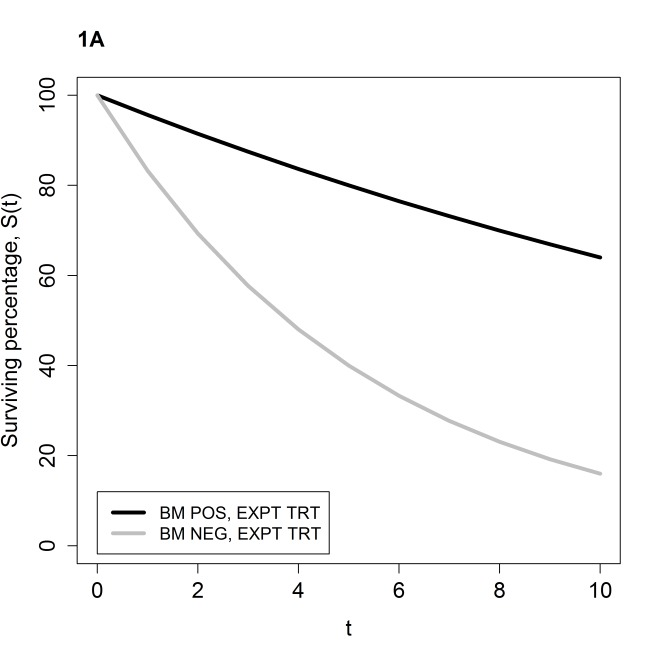
\includegraphics[width=0.475\textwidth]{prognostic.jpg}
    \hfill
    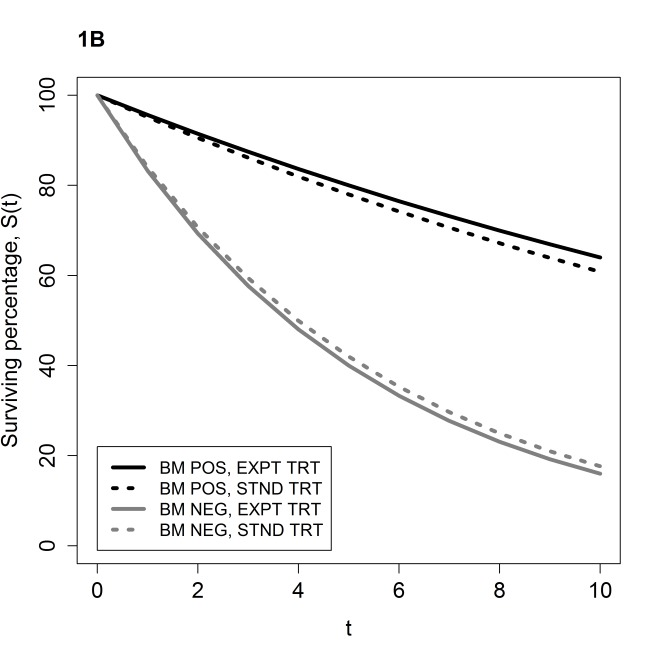
\includegraphics[width=0.475\textwidth]{prognostic2.jpg}
 \end{figure}

\end{frame}


\begin{frame}
\frametitle{Predictive Biomarkers}

\begin{figure}
    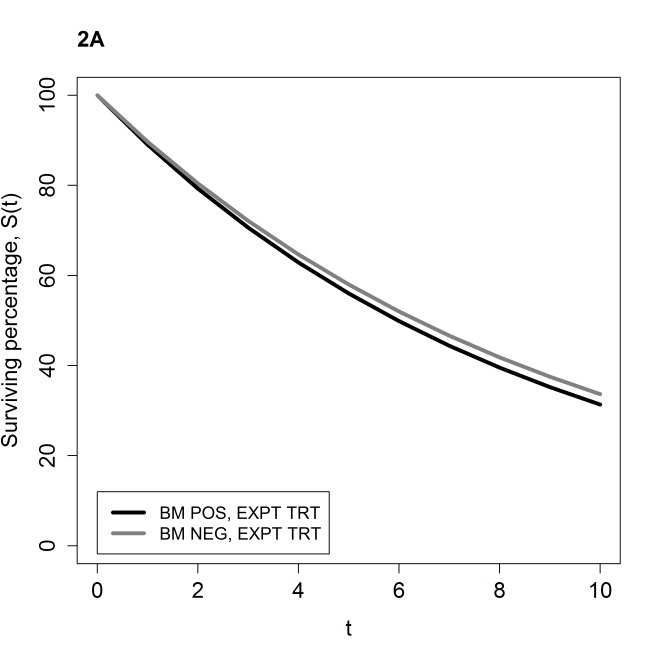
\includegraphics[width=0.475\textwidth]{predictive3.jpg}
    \hfill
    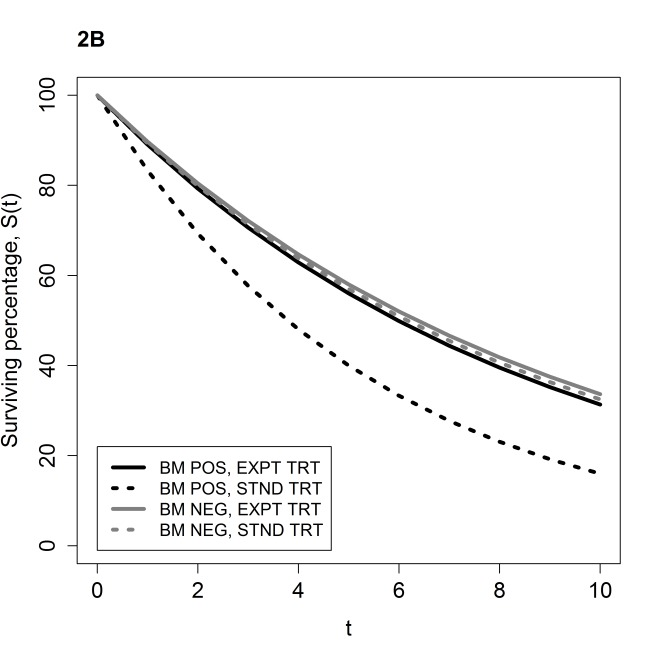
\includegraphics[width=0.475\textwidth]{predictive4.jpg}
 \end{figure}

\end{frame}


%------------------------------------------------


\subsection{Why not regression trees?}

\begin{frame}
\frametitle{Tree-based Methods}

Regression trees GUIDE\cite{loh}:

\begin{itemize}
    \item piecewise-linear Model
    \item examine residual patterns for each treatment level
\end{itemize}

Cannot repeat even the most naive simulation in GUIDE paper.\\~

Reason: limited sample size. Even two splits will results in small sample size in each branch. The results would be highly unstable. Tree-based method is not appropriate
to clinical trial dataset and identify prognostic and predictive biomarkers.

\end{frame}

\section{Methods}

\begin{frame}
\frametitle{Ordinary Linear Model}

$$Y=X\beta + W\tau + G\alpha + W\otimes G \gamma+\epsilon$$

\begin{itemize}
    \item $X$: Baseline variables
    \item $W$: Treatment variables
    \item $G$: Main effects of genes, i.e. expression levels, SNP or mutation
    \item $W\otimes G$: Interaction effects of genes and treatment
    \item $\epsilon$: Random errors
\end{itemize}
\end{frame}

\begin{frame}
\frametitle{Group lasso}

We choose group lasso for its ability to 

\begin{itemize}
    \item handle high dimensional data
    \item allow hierarchical structure
\end{itemize}

However, the current group lasso based methods

\begin{itemize}
    \item penalize on all parameters
    \item have no efficient adaptive penalty weights
    \item do not specifically target on patients treatment subgroup identification
\end{itemize}

\end{frame}

\begin{frame}
\frametitle{Loss Function}

We assume the hierarchical relationship between prognostic biomarkers and predictive biomarkers, 
that is a predictive biomarker should be a prognostic biomarker.\\~
The loss function is

$$\min_{\theta} f(\theta|Y,X,W,G)+ g(\theta)$$

 where $$ g(\theta)=\lambda \sum_i \phi_i^I |\gamma_i| + \lambda \sum_i \phi_i^M \sqrt{\alpha_i^2 + \gamma_i^2}$$

where $f(\theta|Y,X,W,G)$ is L-2 loss function, i.e. sum of squared errors for ordinary linear model.\\~

$\theta=(\beta, \tau, \alpha, \gamma)$ is parameter vector.



\end{frame}

\begin{frame}
\frametitle{Loss function for ordinary linear model}

$$\min_{\theta} \parallel Y-(X\beta + W\tau + G\alpha + W\otimes G \gamma) \parallel^2 + \lambda \sum_i \phi_i^I |\gamma_i| + \lambda \sum_i \phi_i^M \sqrt{\alpha_i^2 + \gamma_i^2}$$

Denote $X^{(l)}=[G_l,W\otimes G_l]$ is the $l$th group of the main and interaction effects of gene $l$.
Then we let $$\phi_i^I=\parallel X^{(i)}\parallel_2$$
\end{frame}


\section{Algorithm}

\subsection{Algorithm Workflow}

\begin{frame}
\frametitle{Optimization Stratgies}
\begin{itemize}
\item Fast iterative shrinkage-thresholding algorithm with backtracking\cite{fasta}
\item Adaptive restart for rippling behavior \cite{restart}
\item Adaptive stepsize of cyclic Barzilai-Borwein spectral approach\cite{step}
\item Warm start in cross validation
\end{itemize}

\end{frame}


\begin{frame}
\frametitle{Proximal Operator}
\begin{block}{Definition}
Let $$Q_{\tau_i,g}(x,u)=g(x)+\frac{1}{2\tau}\parallel x-u\parallel^2$$
then the proximal operator is defined as $$\tilde{x}=arg\min Q_{\tau_i,g}(x,u)$$
For convenience, we denote $P_{\tau_i,g}(u)=\tilde{x}$
\end{block}
Remark: Proximal operator is a point that compromises between minimizing $g$ and being near to $u$. 
\end{frame}

\begin{frame}
\frametitle{Algorithm}
\begin{algorithm}[H]
 initialization $x\theta0=0$ or warm start from previous run, $\tau_0=0.1$, stepsize $\eta=0.5$\;
 \While{$i\le k$}{
 $u_{i}=\theta_{i-1}-\tau_i \bigtriangledown f(\theta_{i-1})$
Find the smallest nonnegative integers $s_i$ such that with $\tau_{i}=\eta^{s_{i-1}}\tau_{i-1}$, $(f+g)(P_{\tau_i,g}(u_i))\le  Q_{\tau_i,g}(P_{\tau_i,g}(u_i),u_i)$\;
Then, we compute $x_{i}=P_{\tau_i,g}(u_i)$
And accelarate the computation by setting 
\eIf{$f(\theta_{i}+g(\theta_i))>f(\theta_{i-1})+g(\theta_{i-1})$}{  $\rho_i=1$
   }{
   $\rho_i=\frac{1+\sqrt{1+4\rho_{i-1}^2}}{2}$
  }
  $\theta_i=x_i+(\frac{\rho_{i-1}-1}{\rho_i})(x_i-x_{i-1})$ and find $\tau_{i+1}$ that $\tau_{i+1}I$ can mimic the Hessian $ \bigtriangledown^2f(x)$
 }
 \caption{Patient Subgroup Identification Group Lasso Algorithm}
\end{algorithm}


\end{frame}

\subsection{Computation of Proximal Operator}


\section{Criteria}

\section{Simulation}



%------------------------------------------------

\begin{frame}
\frametitle{Blocks of Highlighted Text}
\begin{block}{Block 1}
Lorem ipsum dolor sit amet, consectetur adipiscing elit. Integer lectus nisl, ultricies in feugiat rutrum, porttitor sit amet augue. Aliquam ut tortor mauris. Sed volutpat ante purus, quis accumsan dolor.
\end{block}

\begin{block}{Block 2}
Pellentesque sed tellus purus. Class aptent taciti sociosqu ad litora torquent per conubia nostra, per inceptos himenaeos. Vestibulum quis magna at risus dictum tempor eu vitae velit.
\end{block}

\begin{block}{Block 3}
Suspendisse tincidunt sagittis gravida. Curabitur condimentum, enim sed venenatis rutrum, ipsum neque consectetur orci, sed blandit justo nisi ac lacus.
\end{block}
\end{frame}

%------------------------------------------------

\begin{frame}
\frametitle{Multiple Columns}
\begin{columns}[c] % The "c" option specifies centered vertical alignment while the "t" option is used for top vertical alignment

\column{.45\textwidth} % Left column and width
\textbf{Heading}
\begin{enumerate}
\item Statement
\item Explanation
\item Example
\end{enumerate}

\column{.5\textwidth} % Right column and width
Lorem ipsum dolor sit amet, consectetur adipiscing elit. Integer lectus nisl, ultricies in feugiat rutrum, porttitor sit amet augue. Aliquam ut tortor mauris. Sed volutpat ante purus, quis accumsan dolor.

\end{columns}
\end{frame}

%------------------------------------------------
\section{Second Section}
%------------------------------------------------

\begin{frame}
\frametitle{Table}
\begin{table}
\begin{tabular}{l l l}
\toprule
\textbf{Treatments} & \textbf{Response 1} & \textbf{Response 2}\\
\midrule
Treatment 1 & 0.0003262 & 0.562 \\
Treatment 2 & 0.0015681 & 0.910 \\
Treatment 3 & 0.0009271 & 0.296 \\
\bottomrule
\end{tabular}
\caption{Table caption}
\end{table}
\end{frame}

%------------------------------------------------

\begin{frame}
\frametitle{Theorem}
\begin{theorem}[Mass--energy equivalence]
$E = mc^2$
\end{theorem}
\end{frame}

%------------------------------------------------

\begin{frame}[fragile] % Need to use the fragile option when verbatim is used in the slide
\frametitle{Verbatim}
\begin{example}[Theorem Slide Code]
\begin{verbatim}
\begin{frame}
\frametitle{Theorem}
\begin{theorem}[Mass--energy equivalence]
$E = mc^2$
\end{theorem}
\end{frame}\end{verbatim}
\end{example}
\end{frame}




%------------------------------------------------

\begin{frame}
\frametitle{References}
\footnotesize{
\begin{thebibliography}{99} % Beamer does not support BibTeX so references must be inserted manually as below
\bibitem[Loh, 2018]{loh} Loh, Wei‐Yin, Michael Man, and Shuaicheng Wang.  
\newblock "Subgroups from regression trees with adjustment for prognostic effects and postselection inference."
\newblock \emph{Statistics in medicine} (2018).

\bibitem[Beck and Teboulle, 2009]{fasta} Beck, Amir, and Marc Teboulle.
\newblock "A fast iterative shrinkage-thresholding algorithm for linear inverse problems."
\newblock \emph{ SIAM journal on imaging sciences 2.1 (2009): 183-202.  } (2009).

\bibitem[Wright, 2009]{step} Wright, Stephen J., Robert D. Nowak, and Mário AT Figueiredo.
 \newblock "Sparse reconstruction by separable approximation." 
\newblock \emph{IEEE Transactions on Signal Processing 57.7 : 2479-2493.}(2009)

\bibitem[O’Donoghuet and Candes, 2009]{restart} O’Donoghue, B., and E. Candes. 
\newblock  "Adaptive restart for accelerated gradient schemes." 
\newblock \emph{Foundations of computational mathematics 15.3: 715-732.} (2015)

\end{thebibliography}

}
\end{frame}

%------------------------------------------------

\begin{frame}
\Huge{\centerline{The End}}
\end{frame}

%----------------------------------------------------------------------------------------

\end{document} 